\clearpage

\begin{appendix}
\section{Sets of IADS sounds used in Experiment 1: Valence Positive,
Neutral,
Negative}\label{sets-of-iads-sounds-used-in-experiment-1-valence-positive-neutral-negative}

\begin{table}[h]
\begin{center}
\begin{threeparttable}
\caption{\label{tab:appendix_table}Sound-Nr. (Bradley \& Lang, 2007)}
\begin{tabular}{ccc}
\toprule
Positive & \multicolumn{1}{c}{Neutral} & \multicolumn{1}{c}{Negative}\\
\midrule
110 & 109 & 278\\
172 & 171 & 279\\
725 & 206 & 285\\
809 & 221 & 296\\
810 & 270 & 501\\
811 & 365 & 624\\
815 & 367 & 625\\
816 & 368 & 711\\
817 & 375 & 712\\
820 & 722 & 719\\
\bottomrule
\end{tabular}
\end{threeparttable}
\end{center}
\end{table}

\clearpage

\section{Priors for the Bayesian logistic mixed effects regression
models of two-alternative forced choice
responses}\label{priors-for-the-bayesian-logistic-mixed-effects-regression-models-of-two-alternative-forced-choice-responses}

\begin{figure}[!h]
\centering
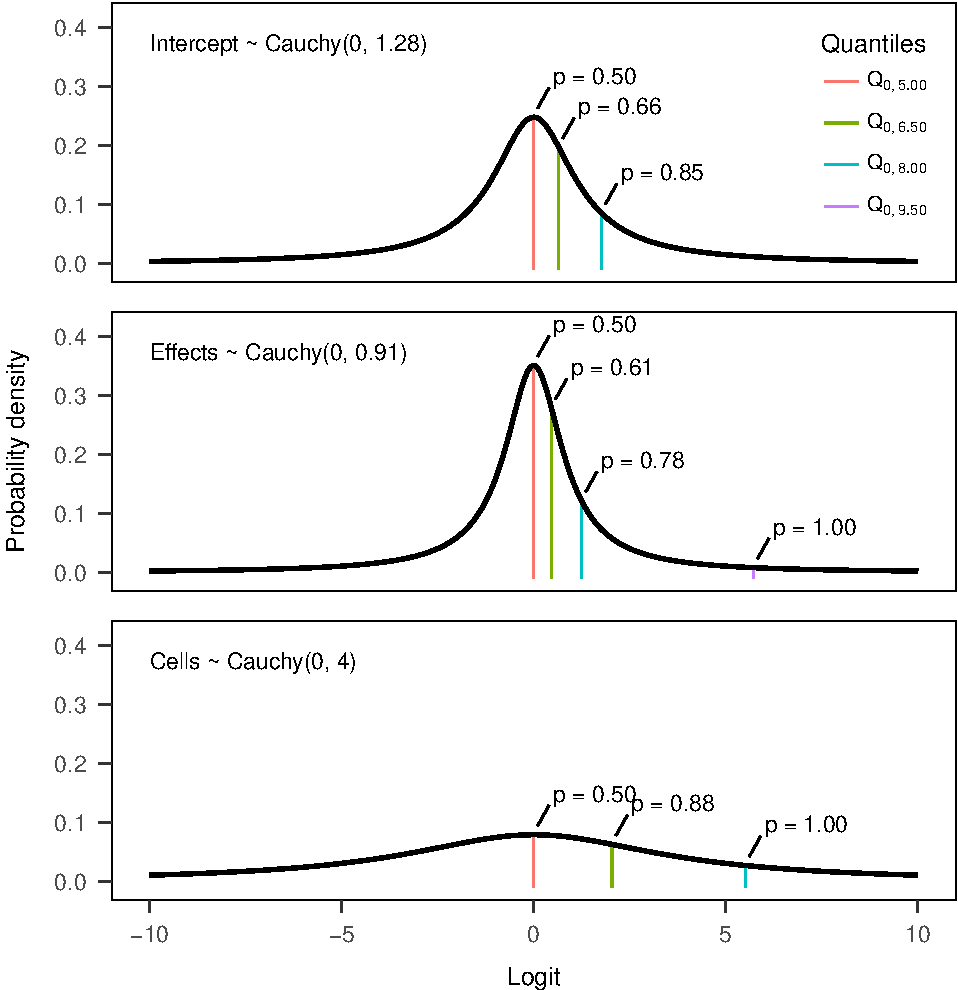
\includegraphics{Chapter02_files/figure-latex/appendix-figure-1.pdf}
\caption{(\#fig:appendix-figure)Priors for the Bayesian logistic mixed
effects regression models of two-alternative forced choice responses.
Colored lines represent distribution quantiles; annoted probabilities
represent the resulting probability of choosing a positively paired CS
starting from chance level (p = 0.5).}
\end{figure}

\clearpage

\section{Mean CS visibility (Experiment 2 and Experiment
3)}\label{mean-cs-visibility-experiment-2-and-experiment-3}

Mean Visibility scores of each CS in Experiment 2 (chance level = .250,
\(N = 37\)) and pilot of Experiment 3 (chance level = .125, \(N = 7\))
and the presentation time for each stimulus as used in Experiment 3.

\begin{table}[h]
\begin{center}
\begin{threeparttable}
\caption{\label{tab:appendix_table2}Mean CS visibility}
\begin{tabular}{cccc}
\toprule
CS & \multicolumn{1}{c}{Visibility Study 2} & \multicolumn{1}{c}{Visibility Pilot} & \multicolumn{1}{c}{Set}\\
\midrule
03.png & .512 & .400 & 1000 ms\\
08.png & .540 & .329 & 1000 ms\\
14.png & .900 & .657 & 1000 ms\\
22.png & .475 & .400 & 1000 ms\\
04.png & .438 & .200 & 20 ms\\
20.png & .400 & .271 & 20 ms\\
50.png & .356 & .129 & 20 ms\\
51.png & .423 & .243 & 20 ms\\
\bottomrule
\end{tabular}
\end{threeparttable}
\end{center}
\end{table}
\end{appendix}
